\section{Methods}

\subsection{Pipeline}
%overview
The tool is implemented as a python package responsible for running the pipeline and conducting supporting analysis. 
The execution of the pipeline to construct a hRIN represents the primary responsibility of the python object and must be ran after object initialization to perform any useful subsequent action on a hRIN. % Would be useful to load hRIN from file.

An overview of the pipeline steps are as follows:
\begin{enumerate}
	\item The pipeline is initiated for a query protein chain identified in a CIF file or a list representing a family of homolog chains is provided by the user.
	\item For a query chain, AA sequence is used as a query for a BLAST homolgy search of either the AlphaFold or PDB database.
	\item Retrieve Structures for homolog proteins.
	\item Multiply align sequences of homolog chains.
	\item Predict non-covalent interactions for each structure with RING.
	\item Synthesize homolog RINs with alignment information to create homology-aware hRIN.
\end{enumerate}


\subsection{Initiation}
The construction of the hRIN is initiated on either a user-chosen query chain or a user supplied family of structure.
In the former situation, the query chain is taken to be a representative example of the protein family - the subject of study that will form the basis of the homolog search and construction of the Interaction network.
To begin, The user supplies a Crystallographic Information File (CIF) that contains the physical information about the query chain. From this file the query polypeptide sequence is extracted and processed to address potential non-standard or unknown residues present in the sequence. Specifically, CIF files will contain a \emph{canonical sequence} for the chain that is the result of some rudimentary processing, simplifying non-standard residues. 
In the ladder case, the pipeline supports analysis of a user defined of protein chains. In this case, the user gives a list of structures which are known a priori to contain homolog chains, forgoing the need for a homolgy search. The user must additionally supply a list identifying which chains withing the structures are the homologs to be considered for the construction of the hRIN (by their internal CIF chain identifiers: label\_asym\_id) in the form of a tsv file containing the name of the structure and the chain ID.

\subsection{Homology Search}
With the query sequence extracted, it is used to perform a homology search with protein-BLAST. The user has the choice to perform this search over either the database of UniProt predictions or the Protein Databank (PDB). 
These database differ in their distribution of contained sequences - with the protein databanks around XXXX protein sequences over XXXX structures representing a notably more biased population than uniprots XXXX protein sequences. 
However, the next step is to automatically download structures for the returned homolog sequences. Metadata describing the map of sequences to their homolog chains in corresponding structures as well as matched regions from the BLAST results are maintained and used for the later construction of the final hRIN.
% Mention BLAST default parameters

\subsection{Structure Retrieval}
%% Not sure if this should go in homolgy search or structure retreival section - it spans both
%% Need the extened information about each database
Due to unreliable experimental structure availability for all of uniprot, choosing to perform the homolog search over the larger database will necessitate that homolog structures be retrieved from the database of AlphaFold2 predictions, which has the notable limitation of contain structures for only a single protein chain. Where searching for sequences over the PDB will result in the pipeline downloading the corresponding experimental structures. These may contain comples of protein chains, other polymers (such as nucleotides) and Ligands. This permits many potential useful analyses. % But has the limitation of...

Once homolog structures are collected, some basic filtering is performed to ensure CIF structures are not malformed, as is sometimes the case in the PDB, preventing the running of RING due to missing secondary structure information, for example. % Information not needed
The peptide sequences of each homolog chain are extracted from the structure. This ensures parody with information contained in the hRIN and the component structures used for its construction, thus avoiding issues caused by out of data BLAST databases and updated PDB/UniProt entries can causing discrepancies. 
Discussion of the different structure databases can be seen in Section \ref{sec:DB-survey}.

In later sections, we regularly refer to a family of structures wich to take to mean the set of structures returned by this process. \todo{finish}

 contains a what we regularly refer to as a \emph{homolog chain} that corresponds to the a sequences identified during the homology search due to its high sequence similarity to the query sequence. In addition to the \emph{homolog chain}, structures in the family, if retrieved from the PDB, are commonly complexes of many entities. It is common that a complex may contain many homolog chains, but we will refer to entities that are not homologous to the query sequence as \emph{non-homolog entities}. These entities are further categorized in Subsection \ref{subsec:node-types}.

\subsection{Sequence Alignement}
% are only blast regions used? - no
% Clustal Omega
The full chain sequences resulting from the operation (not just the sub-sequences returned by BLAST) are aligned into a multiple sequence alignment (MSA) using clustal$\Omega$. This MSA is later used for the identification of nodes within the hRIN.

% MSA figure
Multiple Sequence Alignments function to identify families of corresponding residues in many sequences.
They assume 

\subsection{RING}
Running RING on each homolog structure results in a family of RINs. However, sequence variations across the homolog chains mean that a homology-aware method for synthesizing their information is necessary for the construction of a hRIN. To do this nodes are either defined to be a family of homologous residues or, or a set of non-homolog entities defined across the set of structures. This requires a system of maps relating residues identified in structures as well as indices in BLAST and RING output to columns in the MSA. Non-homolog chain entities are mapped to nodes in the hRIN through a parallel process. The details of node definition are described in Section \ref{sec:hRIN} and Subsection \ref{subsec:node-types}.

\subsection{hRIN Synthesis} % possibly merge into RING subsection.
The final step in the core of the Ring Homology pipeline is the synthesis of the hRIN from previously collected information. The most import aspects of this process include merging homology information from the BLAST search, alignment information from Clustal$\Omega$, and interaction information from RING.




\section{Homology Database}
\label{sec:DB-survey}
% Need to find correct place to discuss AF vs PDB
\subsection{AlphaFold}
AlphaFold is model for predicting the 3D structure of a protein chain given its amino-acid sequence, a challenging and long standing problem in bioinformatatics. AlphaFold2's predictions are renown for their high accuracy, and have proven transformative for the field \cite{alphafold}. 
AlphaFold2 has the notable restriction that predictions are formed for only a single protein chain, not entire complexes of multiple protein chains or ligands - non-polymer structures with which a protein chain is known to bind or interact.  They tend to be of high functional significance, and the subject of many analyses. Ligands are commonly resolved in experimental methods catalogued in the PDB like MNR or X-ray crystallography.
AlphaFold3 predictions include protein complexes and protein-peptide interactions, but have yet to be made widely available for all UniProt sequences via a database.

\subsection{Protein Data Bank (PDB)}
%Inter-chain Contacts
%nucleotide binding

\section{Homology Residue Interaction Network - hRIN}
\label{sec:hRIN}
We use the term Homology Interaction Network (hRIN) to refer to homology enriched RINs.
It should be noted that nodes witin the hRIN do not identify individual residues as they do in typical RINs. Rather, they generally correspond to families of residues as identified by columns in the MSA. In other works this similar concepts of using an MSA to synthasise a set of RINs are called Key Interaction Networks (KINs) \cite{Yehorova2024}. 
\subsection{Contact Conservation}
\label{subsec:def-conservation}
On of the key aspects of homology information encoded to hRINs are edges weighted with the probability or conservation score. This value captures the propensity of an interaction represented by an edge being present in any given member chain of the protein family. 
This required developing different notions of \emph{contact conservation} that can be interchanged depending on the needs of the user. 
The first, more basic, definition simply normalizes the number of observed interactions of a given type for a given pair of nodes by the number of homolog structures in the family. That is, for residue nodes $u,v \in N$ and interaction type $\xi\in\{\texttt{VDW}, \texttt{HBOND}, ...\}$ 
\footnote{The HomologyRing tool supports calculating conservation socres for multiple interaction types at once to support analysis requiring queries selecting multiple interaction types of interest. It only requires that conservation scores also be normalized by the number of selected interactions.} 
(see appendix \ref{appendix:RING-inter}) , we define:
$$p_\xi(u,v) = \frac{1}{|H|} \sum\limits_{x \in H} I_{\xi}(u, v, x)$$ 
where $N$ is the number of homolog structures in the family and $I_\xi$ is simply the indicator function: returning $1$ if nodes $u$ and $v$ are connected by an edge of type $\xi$, else $0$. This does well to normalize interaction counts to probabilities, but has the effect of diminishing some interactions conservation score when it may, in fact, not even be possible in every structure. This is because some nodes may represent families of families of residues given by columns of the MSA with low occupancy, meaning they have gaps or no corresponding residue for some structures. Given the variation seen in the PDB for both indels in sequences, and entities present in complexes, it may be undesirable to penalize such situations for some analyses. To address this, we provide an alternative formulation of conservation:
$$p_\xi(u,v)=\sum\limits_{x\in H}\frac{I_\xi(u,v,x)}{I_\text{non-gap}(u,x) \cdot I_\text{non-gap}(v,x)}$$
\subsection{Inter-Chain \& Ligand Node Identification}
\label{subsec:node-types}
Identifying nodes by families of residues given by columns of the MSA works well for nodes associated with residues in the query structure. However, many structures in the PDB contain a complex of multiple \emph{entities} and many potential analyses performed with RIN concern the interaction of a complex of multiple protein chains and ligands. 
In this context \emph{entity} refers to a structural unit with in structure files. They may be polymer chains (protein or nucleotide) or ligands. \todo{Breifly mention the EIDN system.}
Ligands are small non-polymer molecules, ions or other chemical entities that bind or otherwise interacting with sites of a peptide structure. These can be endogenous molecules like co-factors or signaling molecules.
We make the distinguish primary types of entities for our analysis: protein chains referring and other non-peptide compounds (including nucleotide polymers like DNA and RNA) as ligands. 
With this distinction we classify an edge in a hRIN depending on the entities the nodes the edges connect span. An edge that connects to residues within the same protein chain is referred to as an \emph{intra-chain} edge or interaction. 
Should an edge connect nodes in different protein chains, it is said to \emph{inter-chain}. Finally, an edge connecting a protein chain to a ligand are referred to as \emph{ligand} interactions. 
For the purposes of our analysis we only consider intra-chain contacts to be interactions within chains in the set of homolog proteins, not contacts within chains said proteins may be in contact with. The reasons for this are discussed later in this section.
Furthermore, interactions between non-homolog chains and ligands, and are not included in constructed hRINs. % This choice is not justified by anything other than it would have been annoying to implement. And would be potentially useful for analysis.


When observing the structures within the PDB for a set of homologs it is common to see closely related chains in complex with varying types and quantities of entities across many examples. 
Graphically encoding information of all entities into a homolgy-aware network is challenging. 
There is generally no guarantee that entities present complexes containing a homolog chain in the PDB can be neatly mapped into families across all structures. Given this variability, attempting to encode information about all residues in all present protein in a family of complexes can result in a network that is quite complicated and fails to provide a useful characterization of the family. 

To address this issue we implement a system of identifying corresponding entities across structures returned by the homology search - both protein chains and Ligand compounds. These entities are identified in all structures returned by the homology search. % give a name to this family of structures



With this in mind we can provide a mathematically rigorous definition of the hRIN object that proves useful in later analysis.
In practice, there is much information contained within the nodes of an hRIN, including: 3D position information, consensus residue, residue type.



\section{Analysis Tools}
\subsection{User Defined Queries}
\label{sec:queries}
Given the wide and diverse set of analyses once could potential want to perform on interactions within a protein family, HomologyRing supports users providing a custom query, allowing for the creation and analysis of a sub graph of the initial hRIN created by the pipeline. This sub-hRIN is defined by 3 primary parameters: \texttt{interaction type}, \texttt{interaction class}, and \texttt{region}. 
Filters on \texttt{interaction type} refers to the specific kind of interaction reported by RING. These are listed and described in Appendix \ref{appendix:RING-inter}. This allows users to create a subgraph from a subset of edges of given types.
The different types of non-covalent interactions see different distributions within the PDB. 
Much of the disparity can be attributed to some interactions like \texttt{IONIC} and \texttt{PIPISTACK} may only occur between a specific subset of amino acid residues, but the different interactions are seen to be associated with different structural and functional features. 
RINs constructed from all possible interaction types tend to be quite dense, primarily as a consequence of prolific nature of interactions like \texttt{VDW} and \texttt{HBOND}. The former Van Der Walls interactions are generally present when two neutral compounds are into close proximity and can be either attractive or repulsive. The ladder hydrogen bonds are most commonly responsible for secondary strcture elements within a strcture such as the formation of alpha-helicies or beta-sheets. 
These tend to be generally well perseved within a family of proteins, but can exhibit notabale conservation and variation at binding sites where the homolog chains interface with either another protein chain or a ligand. A protein family that contais many homologs or paralogs that come in complex with a verity of different entities may have a tendency to exhibit interactions spesific to a given entity. where protein chains that are more consistently observed in the same complex will have these sites conserved. % this belongs somewhere else
We later show this to be the case in an example where a famaly of human DDX paralogs are observed to have conserved intra-chain \texttt{HBOND} interactions at binding sites critical for protein function.
Lastly, Hydrogen bonding is also seen to stabalize tertiary and quatary structure to a less common extent. These interact tend to be more variable in families with greater sequence dissimularity. % unsupported, bad asside.
Some of the more novel interactions such as \texttt{SSBOND} are seen to have significant conservation within a family. \todo{move discussion of this to the RING appendix. Be breif here}

Specification of \texttt{interaction class} allows the user to construct a graph out of a subset of edges conditioned on the entities the edges are between. 
Valid choices are intra-chain, inter-chain, chain-ligand contacts, or all and select the respective edges described in Subsection \ref{subsec:node-types}. 
Intra-chain contacts include interactions and corresponding edges between residues in the same protein chain. Consideration of exclusively these edges enable analysis of secondary and tertiary structure variance and conservation within a family.
Inter-chain contacts refer exclusively interactions with participating residues in different protein chains. At a glance, conservation of contacts can deliver insight into which contacts are key to the binding of protein chains to form ligands.
This enables an analysis of binding domains to gain insight into which residues are evolutionary important for interactions or what adaptations in specific sequences may contribute to specificity in partner binding.

Ligands
Metal-coordination can be essential for structure and contain important functional information about a family of proteins.
Co-factors
DNA/RNA

Finally users may place a filter on nodes to be included in the resulting sub-hRIN.
The default behavior is to perform not filtering and include all nodes.
Regions of interest in a family may be specified by the user to create a sub-hRIN that captures interactions with a set of residue nodes. For example, creating a hRIN for an entire structure may provide a lot irrelevant information when performing an analysis on an inter-chain binding substrate conservation within a family. 
Can specify an occupancy ratio, selecting residue-nodes in the network that correspond to MSA columns that contain above a given threshold of non-gaps. This allows users to quickly discard nodes corresponding to the poorly conserved tails of the MSA that are not representative of the family. 
It should be noted that region filters placed on the nodes are not strict, and should an edge have at least one node in the selected region, the edge and both nodes the edge connects will be included in the resulting hRIN.

\subsection{Contat Mask Plots}
\label{sec:contact-masks}
A very quick means of identifying groups of conserved interactions within a family of proteins is the use of \emph{contact mask plots}. These display an image of the MSA used to define the residue nodes in the hRIN. Intuition about the characteristics of each family may be gained by the use of CLUSTAL colors which encodes physio-chemical properties of different residues into color. On top of this is a binary mask indicating that the residue in a given structure and residue family participate in an interaction that matches the users query.



\subsection{Contact Conservation Plots}
To quantify the conservation of an interaction within a protein family, 
Figure \ref{fig:ex-contact-plot} graphically shows the conservation score as calculated in Section \cite{placeholder}
\begin{figure}[ht] % replace with [H} if position is causing problems.
    \centering
    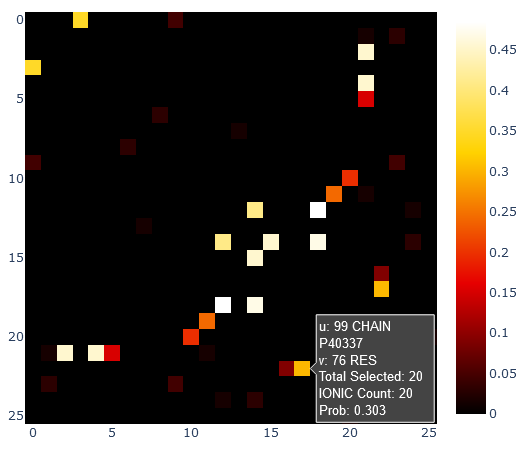
\includegraphics[width=0.5\textwidth]{fig/Contact_conserv.png}
    \caption{Example of \emph{contact conservation plot} showing the scores for \texttt{IONIC} and \texttt{PIPISTACK} interactions for all node types: \texttt{RES}, \texttt{CHAIN}, and \texttt{LIG}.}
    \label{fig:ex-contact-plot}
\end{figure}
\subsection{Co-Evolution of Contacts} % Rename this section, coevolution is not correct
With the importance of non-covalent interactions for conformal and functional properties of a protein, a reasonable analysis task is to analyze the conservation and specificity of interactions witin a family by observing the presence of interactions within spesific homolog structures. To achieve this, we provide a means means of classifying structures into a pseudo-taxonomy, grouping structures based on homology-aware RIN similarity. 
Typically, evolutionary relationships can be inferred by sequence similarity: using disparities between multiple residue sequences to infer the elapsed time since a common ancestor. Further structure is given to these relationships by organizing individuals into a tree to map their relationships. We utilize this concept to compare and group structures based not on sequence similarity, but rather the similarity of their respective RINs.

At the core of this approach is a means of quantifying the dissimilarity of RINs based on their graph definition and the node maps integral to hRINs.
Given a hRIN $G = (N, E)$, for homolog protein structure $x$ we define $E_x \subseteq E$ to be the set of edges observed in structure $x$. 
We continue to define the edge difference set, $D_{x,y} \subseteq E$ for two homolog structures $x$ and $y$ to be the set of edges present in either $x$ or $y$ exclusively. This can otherwise be thought of as the symmetric difference of the subgraph edgesets:
$$
D_{x,y} =(E_x\backslash E_y)\cup(E_y\backslash E_x)= E_{x}\oplus E_y
$$
Visulization of this operator is shown in Figure \ref{fig:graph-diff}. Observe, edges are considered to be shared between two graphs if their incident nodes have the same labels. We are able adapt this notion thanks to the node maps created with the MSA, and may avoid using more complex and computationally expensive notions of graph similarity. Additionally, the result may have node set of the result will be the union of the two graphs. 
\begin{figure}[ht] % replace with [H} if position is causing problems.
    \centering
    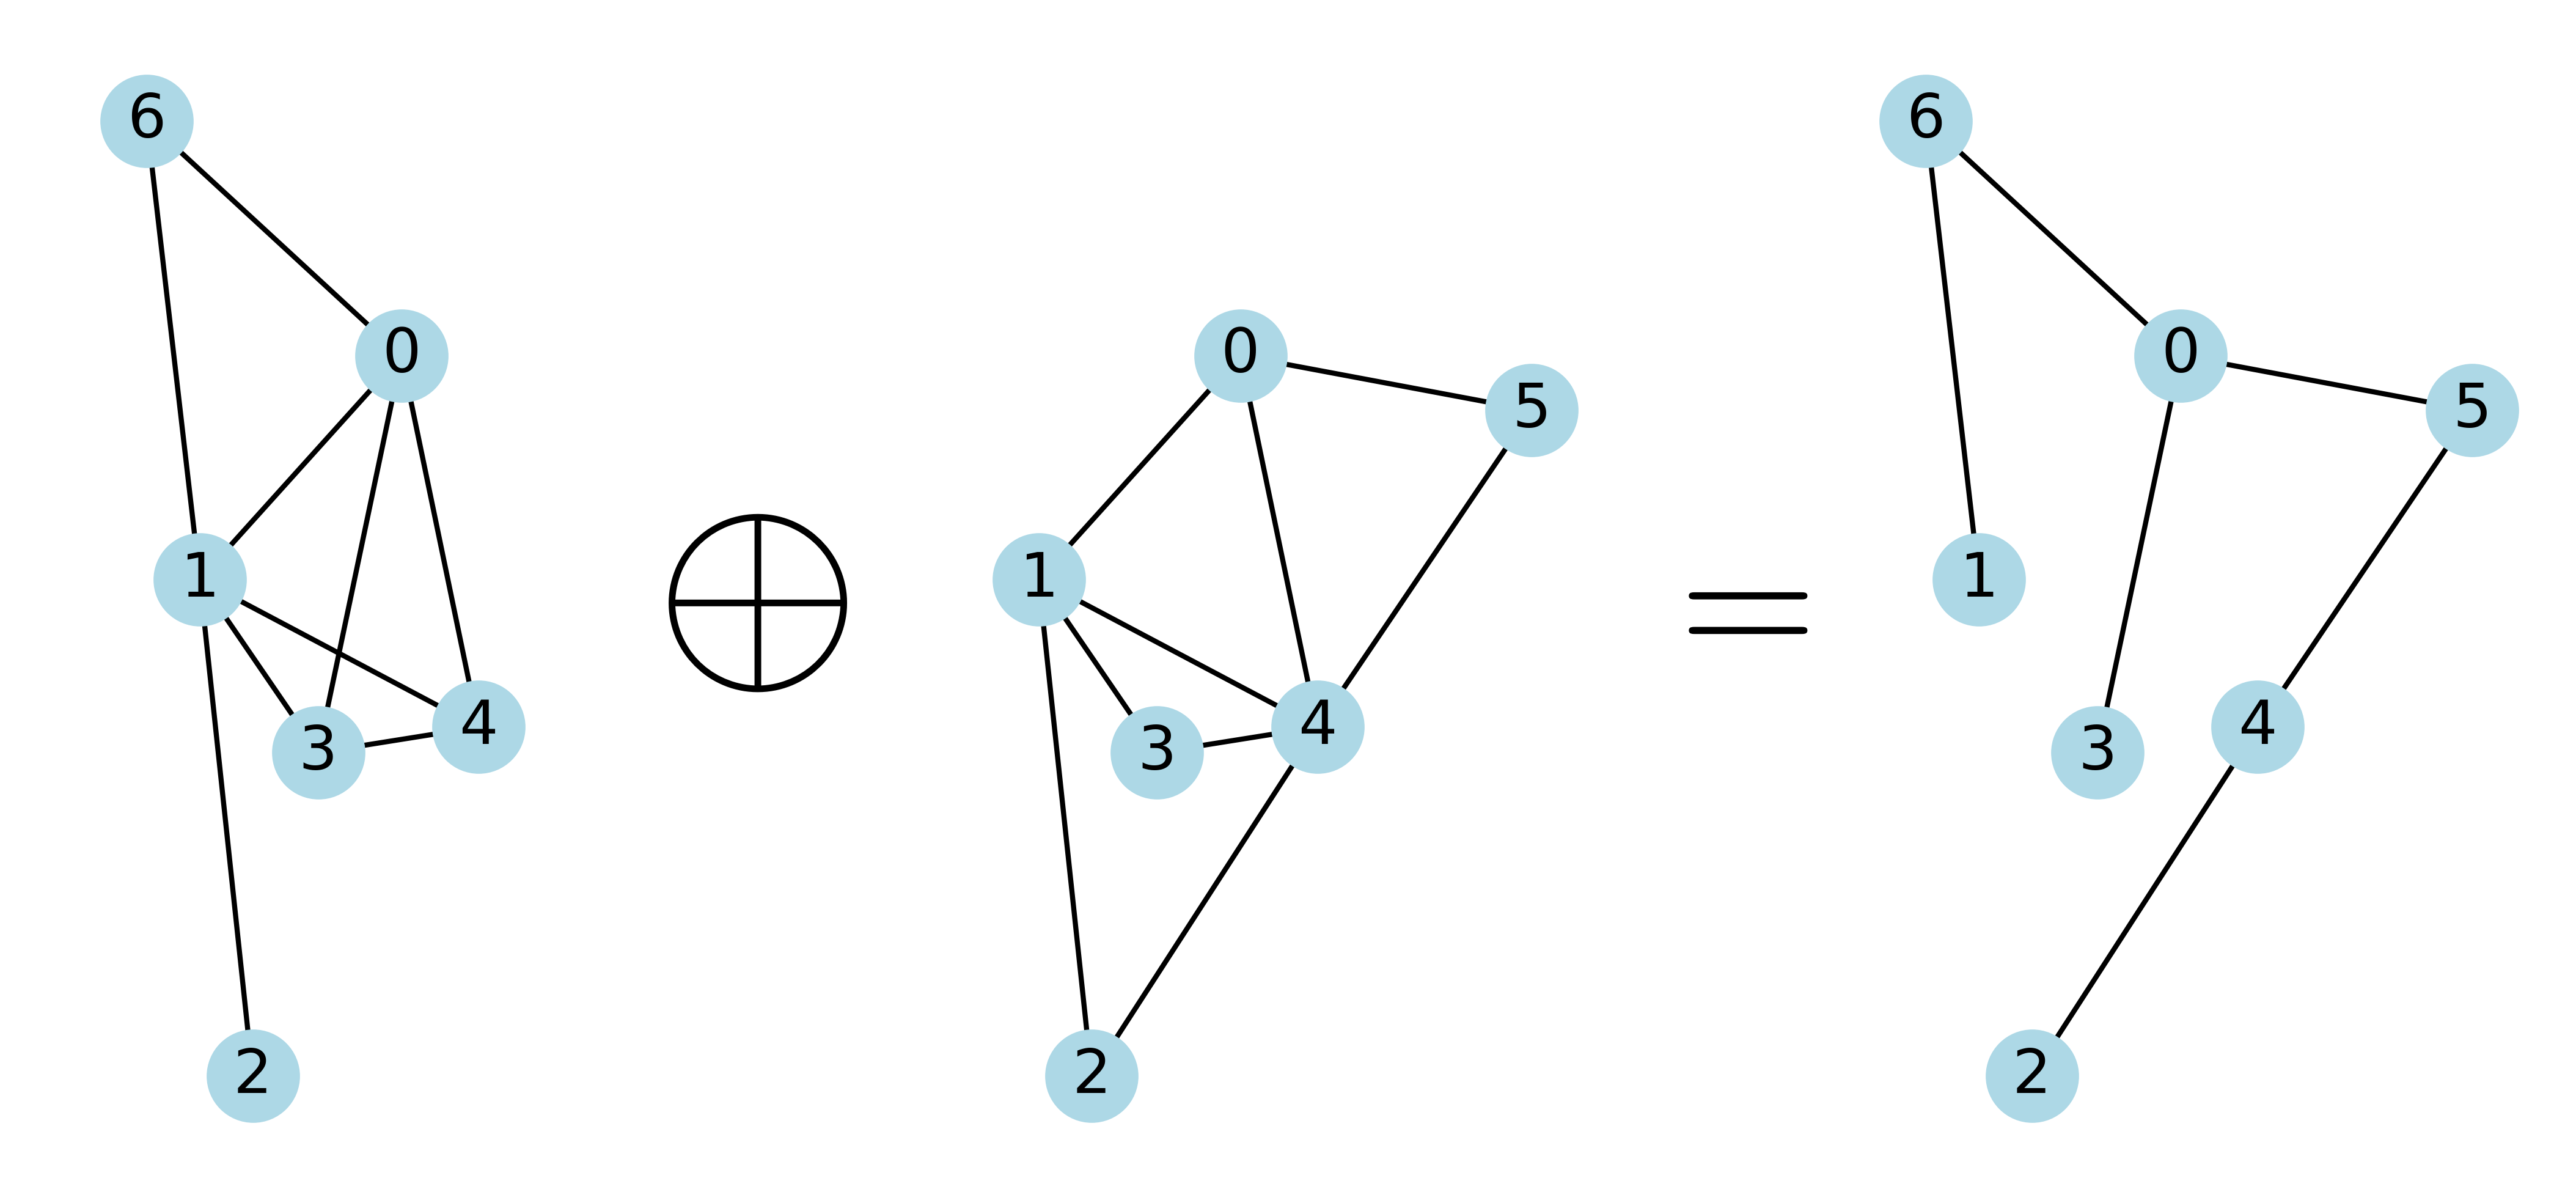
\includegraphics[width=0.5\textwidth]{fig/graph-diff.png}
    \caption{Example of the graph \emph{Symmetric Difference} (XOR) operator on graphs.}
    % For $A,B \subseteq G$, we consider edges in $A \oplus B \subseteq G$ to contribute to the distance between $A$ and $B$.
    \label{fig:graph-diff}
\end{figure}

With this we define both a unweighted and weighted pseudo-distance\footnote{This cannot be called a true distance metric, as the triangle inequality does not neccessarially hold. However, does not represent a significant issue for practical issue.} to quantify the dissimilarity of homolog chains based on the interactions the admit.
$$
d(x,y) = |D_{x,y}| \quad\text{or}\quad d(x,y) = \sum\limits_{e\in D_{x,y}} p(e)
$$
This is also referred to as Hamming distance, though it is worth noting that the weighted version in this context differes from most uses of the Weighted Hamming Distance, where the difference in edge wieghts between the two different graphs are summed. Here the edges, if they are shared between the two subgraphs, will have the same weights, and will not contribute to the distance.

The ladder weighted variant will penalize more discrepancies of highly conserved edges - considering homologs with edges , where the unweighted variant  considers only the number of unshared edges significant. 
The type of analysis being performed should inform the choice between the two. Studies of contact conservation will desire that structures that admit highly conserved edges will be grouped closer together in the resulting taxonomy, while studies of specificity will value shared novel or uncommon edges more important when grouping structures.

With the distance metric defined, the sequences organized into a rooted tree, or deprogram, using the popular unweighted pair group method with arithmetic mean (UPGMA) method. 
This is an iterative method, employed here to create a heigharchial clustering of structures based on non-covalent interactions of interest. At each iteration, the method defines a distance between groups of examples based on the average inter-group distance:
$$d(X,Y) = \frac{1}{|X||Y|} \sum\limits_{x\in X} \sum\limits_{y\in Y} d(x,y)$$

This is referred to a pseudo-taxonomy because it does not aim to capture inferred evolutionary relationships, rather group structures based on the similarity of the non-covalent interactions the admit. This is useful for finding patters of contact conservation or specificity. For example: conformal variations of a protein complex may give rise groups of variably conserved interactions. 
\todo{replace fig with example dendrogram}
\begin{figure}[ht] % replace with [H} if position is causing problems.
    \centering
    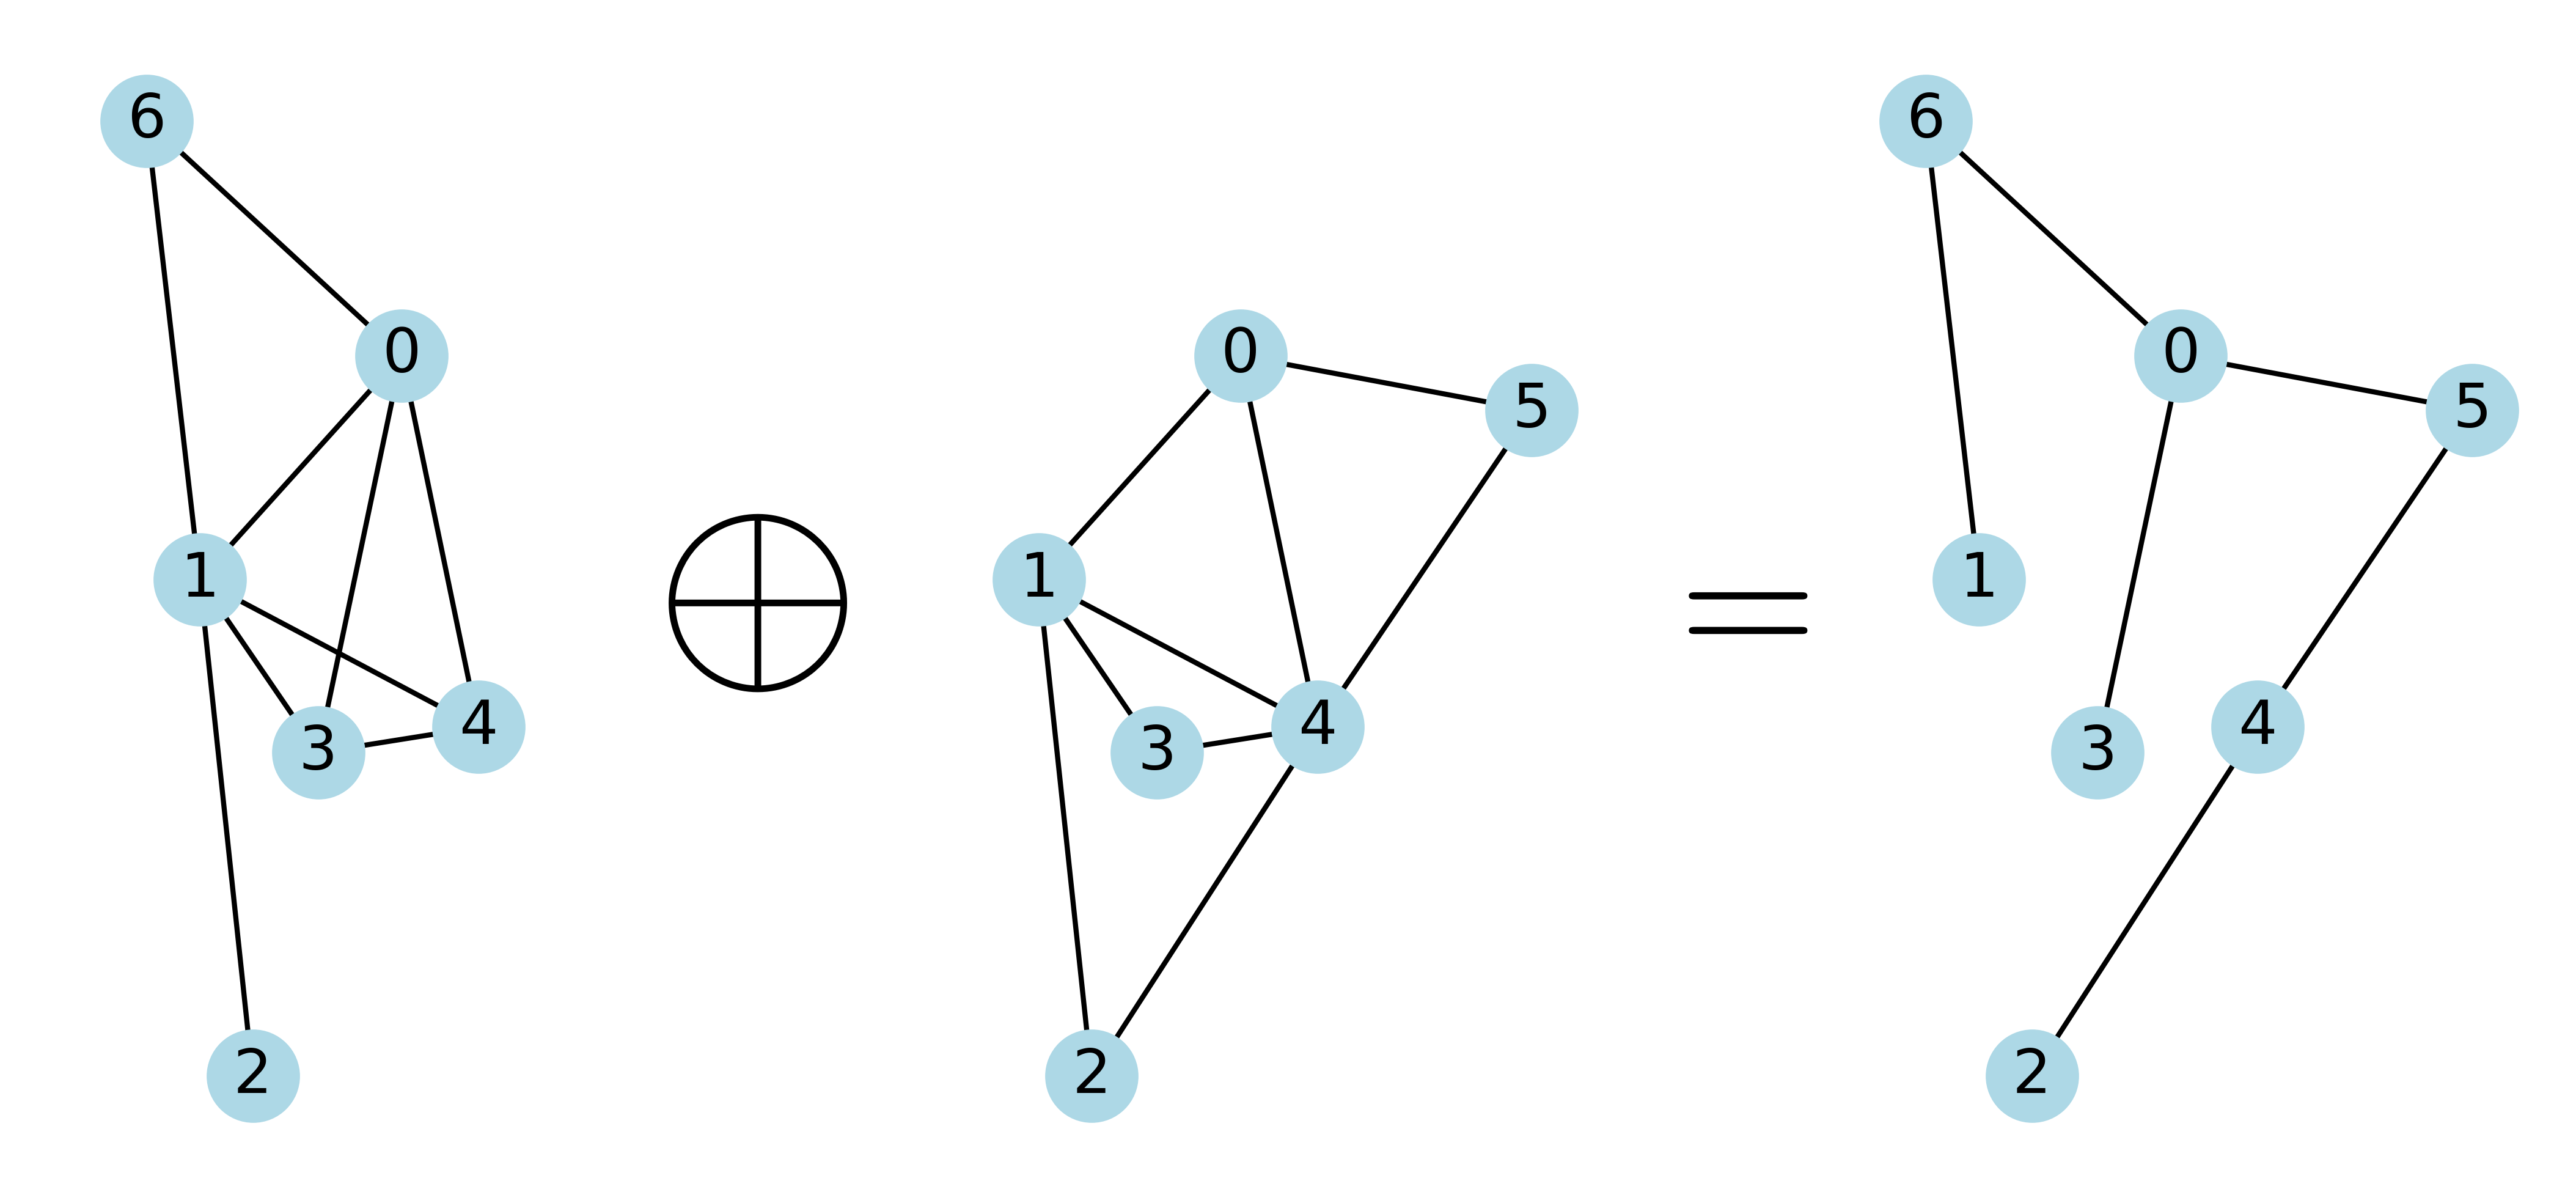
\includegraphics[width=0.5\textwidth]{fig/graph-diff.png}
    \caption{Example of dentrogram created to created structural similarity based on residue interactions.}
    \label{fig:struct-dendro}
\end{figure}